\documentclass [a4paper,12pt] {article}
\usepackage[utf8]{inputenc}
\usepackage[french]{babel} % francisation                                                                                                                                  
\usepackage{graphicx}
\usepackage[nottoc, notlof, notlot]{tocbibind}
\author{Manson Tomy\\Mestreau Nicolas\\Ridel Fabien\\Wen Jun \vspace*{1cm} \\Client :\\Jérémy Laviole}
\date{}
\title{\rule{\linewidth} {1pt}\\\textbf{Extraction et analyse d’image}\\ Projet d'étude et de Développement\\\rule{\linewidth} {1pt}}
%\bibliographystyle{ieeetr}
\bibliographystyle{plain}
%%%% debut macro %%%%
\makeatletter
\def\captionof#1#2{{\def\@captype{#1}#2}}
\makeatother
%%%% fin macro %%%%
\begin{document}

\maketitle
\newpage
\tableofcontents

\newpage
\section{Introduction}
\subsection{Présentation}

L'objectif de notre projet d'étude et de développement est de produire une bibliothèque d'extraction et d'analyse d'images à partir d'un flux vidéo. Cette bibliothèque sera utilisée pour des applications de vision par ordinateur.\\

L'extraction d'images consiste à récupérer un espace de dessin dans la vidéo. cet espace de dessin peut être une feuille blanche, entourée par une planche de tags. Au début du projet, une bibliothèque d'extraction (\texttt{ARToolkit}) nous a été fournie. Nous devions donc nous concentrer sur les analyses des images obtenues.\\

Les analyses demandées par ce projet sont de deux types : 
\begin{itemize}
\item Une analyse rapide, sur une image de faible qualité. Le but de cette analyse est de retrouver des formes simples (voir les templates ci-dessous) dans le dessin.
\item Une analyse sur des images de haute qualité. Cette analyse a pour but de détecter les nouveautés dans le dessin.\\
\end{itemize}
Des applications utilisant la bibliothèque sont également à développer, notamment une application de détection de nouveautés dans un dessin, et une application de reconnaissance de formes simples.

\newpage
\section{Objectifs}
\subsection{Cahier des charges}

Dans le but de développer la bibliothèque, nous avons établi un cahier des charges présentant et définissant les trois ensembles de fonctionnalités qui la constitue :
\begin{itemize}
\item Pré-traitement des images
\item Détection des évolutions d'un dessin
\item Reconnaissance des formes dessinées
\end{itemize}

\subsubsection{Pré-traitement}

Tout traitement sur une image nécessite d'effectuer un certain nombre de pré-traitements afin d'améliorer la qualité de cette image. Cette étape a pour but de favoriser l'obtention de bons résultats lors de la phase de traitement.\\

La bibliothèque devra permettre d'appliquer aisément un certain nombre de filtres, notamment :

\begin{description}
\item[Filtre morphologique] Optimisation des methode de template matching;
\item[Binarisation] Permettre de trouver les différences qui existent entre deux images;
\item[Correction de couleur] Balance des blancs, permet d'annuler la coloration globale de l'image, dépendante de l'éclairage de la scène (lumière du jour, lumière artificielle, etc ...);
\item[Filtrage par couleur] Récupérer uniquement les formes dessinées avec une couleur précise.
\end{description}

La bibliothèque devra permettre de developper de nouveau filtres. Tous les filtres devrons pouvoir être utilisés de la même manière afin d'en simplifier l'usage, ils devrons avoir une interface commune.

\clearpage
\subsubsection{Détection des évolutions d'un dessin}

La première fonctionnalité de la bibliothèque est de permettre la récupération de plus haute qualité possible d’un dessin à différents moments. Les moments de prise de vue du dessin seront considérés comme idéaux, pas de mains, ni d'objets dans le champs de prise de vue.

On cherche ici à permettre le développement d'applications permettant d'observer les moments clés de la création d'un dessin sans perturber le travail de l'artiste, c'est à dire, éviter de scanner la feuille.

\paragraph{Performance\protect\footnotemark[1]\\}
La bibliothèque devra permettre l'analyse d'image à une cadence de 2 à 3 images par seconde. Le but ici n'est pas la performance mais bien la qualité de l'analyse.
Les images à traiter seront aquises en haute definition, un minimum de 1080 lignes de 1920 pixels, ce qui correspond à la resolution d'un flux vidéo HDTV 1080p.


\subsubsection{Reconnaissance des formes dessinées}
La deuxième fonctionalité de la bibliothèque est de reconnaitre, dans un flux video, des dessins ou pictogrammes préenregistrés. 

Différentes méthodes pourrons être développées selon que les formes à reconnaitre dans l'image sont simples (p.ex. : un carré, un cercle) ou complexe (p.ex. : un visage).

On utilisera par exemple :

\begin{itemize}
\item Template Matching : Mise en correspondance d'une image avec une image de référence pour la detection de formes simple.
\item Feature detection : Utilisation de caractéristique invariante dans l'image pour la reconnaisance de formes complexe (par exemple: descripteur SURF).
\end{itemize}

\paragraph{Performance\protect\footnotemark[1]\\}
La bibliothèque devra permettre l'analyse d'image à une cadence de 30 à 60 images par seconde. Le but ici est d'effectuer de l'analyse sur un flux vidéo temps réel, de basse qualité.
Les images à traiter seront aquises en basse qulaité, on prendra comme base des vidéos au format vidéo VGA 480 lignes de 640 pixels, ce qui correspond au format VGA.

\footnotetext[1]{Les problématiques de performance sont secondaires, l'objectif principal est de developper une bibliothèque qui fonctionne.}

\clearpage
\subsection{Planning}
Le projet s'est déroulé suivant un planning se découpant en deux phases principales : une phase de préparation et d'organisation du projet et une phase de développement, de tests et de fin de projet.\\

La phase de préparation et d'organisation, présentée dans le diagramme de Gantt ci-après, est divisée en deux tâches :
 \begin{itemize}
 \item \'Etablissement du cahier des charges par l'ensemble du groupe
 \item \'Etude de l'existant. Cette dernière étant subdivisée en deux sous-tâches : 
	 \begin{itemize}
		\item \'Etude des methodes de prétraitements d'image, réalisé par Fabien Ridel et Jun Wen;
		\item \'Etude des méthodes d'extraction de nouveautés et de de reconnaissance de forme dans l'image, réalisé par Tomy Manson et Nicolas Mestreau.
	\end{itemize}
\end{itemize} 

\begin{center}
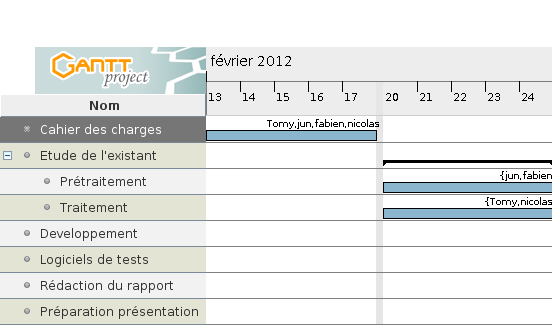
\includegraphics[width=\textwidth]{gantt1.png}
\captionof{figure}{Planning taches préparatoire}
\end{center}

\clearpage
La phase suivante, présentée dans le diagramme de Gantt ci-après, est la phase de développement de la bibliothèque, de programme de démonstration et de tests. Nous incluons dans cette phase la rédaction du rapport et la préparation de la présentation, qui constituent la fin de projet.

\begin{center}
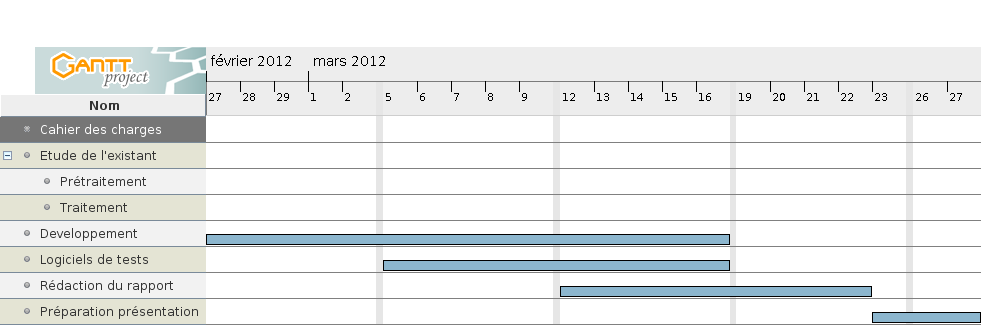
\includegraphics[width=\textwidth]{gantt2.png}
\captionof{figure}{Planning de dévelopement et de fin de projet}
\end{center}

%
%\begin{center}
%\includegraphics[scale=0.15]{spatio_temporal_tracking.png}
%
%\captionof{figure}{Example of a tracking on a spatio-temporal saliency map}
%\end{center}

\newpage
\section{Travail accompli}
\subsection{Architecture logicielle}

\subsection{Choix d'implementation}
template matching fonctionne mais pas bien

filtre ->  patron de conception "patron de méthode" permet d'unifier les comprtement des filtres et factoriser du code
			"factory"

\subsection{Optimisation}

\subsection{Difficultés}

\newpage
\section{Tests et résultats}
\subsection{Presentation des logiciels de test}


\newpage
\section{Conclusion}
En faisant le bilan global de notre projet, on peut dire que l'objectif a été partiellement atteint. Nous avons fourni des interfaces permettant l'utilisation de filtres et de détecteurs. Cependant, des optimisations sont encore possibles, pour atteindre les objectifs de performances définis.\\

Nos logiciels de test montrent que l'idée d'analyser des dessins est pertinente. Nous avons réussi à détecter des pictogrammes simples, et nous avons un résultat acceptable pour la détection de nouveautés.\\

Les différentes pistes qui suivent notre projet sont :
\begin{itemize}
\item Amélioration des détecteurs (notamment instaurer un seuil pour le template matching)
\item Approche par apprentissage automatique pour les détecteurs de formes plus complexes.
\item Utilisation du masque de nouveautés pour effectuer une vectorisation étape par étape du dessin.
\end{itemize}


\clearpage
\bibliography{biblio.bib}


\end{document}
